\documentclass[11pt,a4paper]{article}

\usepackage[margin=0.8in]{geometry}
\usepackage{amsmath}
\usepackage{graphicx}
\usepackage[table]{xcolor}
\usepackage{hyperref}
\usepackage{array}
\usepackage{longtable}
\usepackage{titlesec}
\usepackage{setspace}

\hypersetup{hidelinks}
\setlength{\parskip}{0.45em}
\setlength{\parindent}{0pt}
\renewcommand{\arraystretch}{1.2}
\setlength{\extrarowheight}{2pt}

\definecolor{TitleBlue}{HTML}{153E75}
\definecolor{SoftBlue}{HTML}{EAF2FF}
\definecolor{SoftGray}{HTML}{F5F7FA}
\definecolor{RiskGreen}{HTML}{37B24D}
\definecolor{RiskDkGreen}{HTML}{2B8A3E}
\definecolor{RiskYellow}{HTML}{FEE440}
\definecolor{RiskOrange}{HTML}{FF922B}
\definecolor{RiskRed}{HTML}{F03E3E}
\definecolor{RiskDkRed}{HTML}{C92A2A}

\titleformat{\section}{\large\bfseries\color{TitleBlue}}{\thesection.}{0.5em}{}
\titleformat{\subsection}{\normalsize\bfseries\color{TitleBlue}}{\thesubsection}{0.5em}{}

\begin{document}

\begin{center}
{\LARGE\bfseries\color{TitleBlue} PHC Integrated Digital System}\\[0.3em]
{\Large Groupno\_Lab910}\\[0.6em]
{\large Lab 9 \& 10 Report: Software Metrics and Risk Handling}\\[0.8em]
{\normalsize Bavadiya Yash Kiritbhai \quad Chaitanya Singh \quad Nayan Patidar}\\[0.3em]
{\normalsize IIT Jodhpur}\\[0.8em]
\fcolorbox{TitleBlue}{SoftBlue}{\parbox{0.92\linewidth}{
\textbf{Report intent.} This report tells the project story as one connected narrative: how the PHC system evolved sprint by sprint, what the repository proves today, which metrics matter, where the real risks emerged, and how those risks were already folded back into planning and backlog decisions.}}
\end{center}

\section{Project Story and Evidence Baseline}
The PHC Integrated Digital System started as a documentation-heavy academic project, but by the end of Sprint 5 it had become a working backend platform with authentication, patient records, visit lifecycle management, prescription handling, laboratory flows, billing, appointments, notifications, and admin reporting. That progression matters for this lab because the requested metrics are meaningful only if they are tied to the actual engineering story rather than to abstract estimates.

For this report, we used the current repository as the evidence baseline. The measured story comes from \texttt{README.md}, \texttt{TESTING.md}, \texttt{test\_cases.csv}, \texttt{backend/prisma/schema.prisma}, all backend route and service files, SRS revisions through Version 2.2, and git history from January 15, 2026 to April 3, 2026. The resulting snapshot is:

\begin{center}
\rowcolors{2}{SoftGray}{white}
\begin{tabular}{|p{8cm}|p{4cm}|}
\hline
\rowcolor{SoftBlue}
\textbf{Repository-backed baseline} & \textbf{Measured value} \\
\hline
Production source lines of code & 2859 \\
Backend source lines of code & 2505 \\
Service-layer source lines of code & 1608 \\
Persisted domain models & 20 \\
Implemented API endpoints & 57 \\
Documented categorized test cases & 48 \\
Feature commits in the active project window & 21 \\
\hline
\end{tabular}
\end{center}

The most useful qualitative observation from this baseline is that the project is backend-heavy by design. The service layer contains most of the domain logic, which is exactly what we would expect from a system where correctness, traceability, and role safety matter more than early frontend polish.

\subsection{Late Sprint 5 Closeout Evidence}
Because Sprint 5 was the backend integration sprint, the latest repository evidence is concentrated near the end of March 2026. The sequence below is the corrected chronology used for the tracker and for this report.

\begin{center}
\rowcolors{2}{SoftGray}{white}
\begin{tabular}{|p{1.9cm}|p{2cm}|p{4.1cm}|p{6.7cm}|}
\hline
\rowcolor{SoftBlue}
\textbf{Date} & \textbf{Commit} & \textbf{Sprint 5 item} & \textbf{Meaning in the project story} \\
\hline
2026-03-25 & \texttt{9e3e7c0} & Local LDAP-backed authentication & Converted authentication from the earlier dev fallback approach into a proper local LDAP bind flow for seeded users. \\
\hline
2026-03-25 & \texttt{3fac9c2} & Full-system E2E runner & Added a repository-backed end-to-end validation path across the major backend modules. \\
\hline
2026-03-25 & \texttt{2d7e421} & Sprint 5 integration docs closeout & Synchronized API documentation and backend integration evidence near sprint closeout. \\
\hline
2026-03-25 & \texttt{9182fcc} & Availability notifications & Added doctor unavailability and in-app notification logic, reducing operational ambiguity. \\
\hline
2026-03-24 & \texttt{5ff16c2} & Admin user management & Added administrative account creation, listing, status control, and role updates. \\
\hline
2026-03-24 & \texttt{248d70a} & Usage and attendance reports & Added management-facing reporting endpoints for usage and doctor attendance summaries. \\
\hline
2026-03-24 & \texttt{b66f7f2} & PHC events module & Added event publishing and public event visibility for PHC communication. \\
\hline
2026-03-24 & \texttt{7718df7} & Patient lab report access & Added role-safe patient access to their own laboratory reports. \\
\hline
2026-03-24 & \texttt{f1ef67b} & Lab request detail endpoint & Added single-request detail retrieval with access control checks. \\
\hline
\end{tabular}
\end{center}

\section{Section I: Metrics and Their Meaning}
\subsection{Intermediate COCOMO}
We modeled the project as an \emph{Organic} COCOMO system because the team is small, the stack is familiar, and the product is complex enough to require engineering discipline without becoming an embedded or mission-critical real-time system. Using 2.859 KLOC of production code and an effort adjustment factor derived from reliability, data sensitivity, functional complexity, team capability, and tooling assumptions, we obtained the following result:

\begin{center}
\rowcolors{2}{SoftGray}{white}
\begin{tabular}{|p{7cm}|p{4cm}|}
\hline
\rowcolor{SoftBlue}
\textbf{COCOMO measure} & \textbf{Value} \\
\hline
Mode & Organic \\
KLOC & 2.859 \\
Effort Adjustment Factor (EAF) & 0.786 \\
Estimated effort & 7.58 person-months \\
Estimated schedule & 5.40 months \\
Average staffing & 1.40 persons \\
Productivity & 0.377 KLOC / PM \\
\hline
\end{tabular}
\end{center}

This estimate aligns with the real project story better than it may first appear. The backend has been completed by a small team over a compressed academic schedule, but that happened by deferring frontend work and concentrating effort in the backend first. So the main use of COCOMO here is not to claim exact planning accuracy; it is to show that the system has already crossed the scale of a toy application and sits in the range where architectural discipline matters.

\subsection{Halstead Metric}
Halstead metrics were computed over the backend source files after removing comments and string literals. The purpose was to estimate the size and mental complexity of the implemented codebase.

\begin{center}
\rowcolors{2}{SoftGray}{white}
\begin{tabular}{|p{7cm}|p{4cm}|}
\hline
\rowcolor{SoftBlue}
\textbf{Halstead measure} & \textbf{Value} \\
\hline
Distinct operators \(n_1\) & 55 \\
Distinct operands \(n_2\) & 536 \\
Total operators \(N_1\) & 11799 \\
Total operands \(N_2\) & 4931 \\
Program vocabulary & 591 \\
Program length & 16730 \\
Volume & 154033.35 \\
Difficulty & 252.99 \\
Effort & 38968856.88 \\
Estimated delivered bugs & 51.34 \\
\hline
\end{tabular}
\end{center}

The most important takeaway is not the absolute effort number but what it implies: the backend already has enough vocabulary and domain spread that ad hoc coding would quickly become fragile. That explains why the current layered structure, route-level RBAC, and transaction-protected operations are not optional niceties; they are required to keep the system understandable.

\subsection{Function Point Analysis}
Function Point Analysis was derived from the actual route inventory and database model. Endpoints were classified into external inputs, outputs, and inquiries; Prisma models were treated as internal logical files; LDAP was treated as one external interface file.

\begin{center}
\rowcolors{2}{SoftGray}{white}
\begin{tabular}{|p{3cm}|p{2.2cm}|p{2.2cm}|p{2.4cm}|}
\hline
\rowcolor{SoftBlue}
\textbf{Type} & \textbf{Count} & \textbf{Weight} & \textbf{Contribution} \\
\hline
EI & 28 & 4 & 112 \\
EO & 4 & 5 & 20 \\
EQ & 25 & 4 & 100 \\
ILF & 20 & 10 & 200 \\
EIF & 1 & 5 & 5 \\
\hline
UFP & \multicolumn{3}{c|}{437} \\
VAF & \multicolumn{3}{c|}{1.11} \\
Adjusted FP & \multicolumn{3}{c|}{485.07} \\
\hline
\end{tabular}
\end{center}

This metric reinforces a pattern already visible in the codebase: the system is not just doing CRUD on a few entities. It has workflow-bearing transactions, state transitions, and role-gated behavior. That is exactly why the project narrative should be told as a connected system story and not as disconnected endpoint counts.

\subsection{Cumulative Flow Diagram}
The repository does not store Trello history directly, so the cumulative flow view was reconstructed from the sprint plan in the SRS/README and the actual implementation completion pattern visible in git. The figure below summarizes how planned work transitioned from \emph{To Do} to \emph{In Progress} to \emph{Done} across Sprint 0 to Sprint 5.

\begin{center}
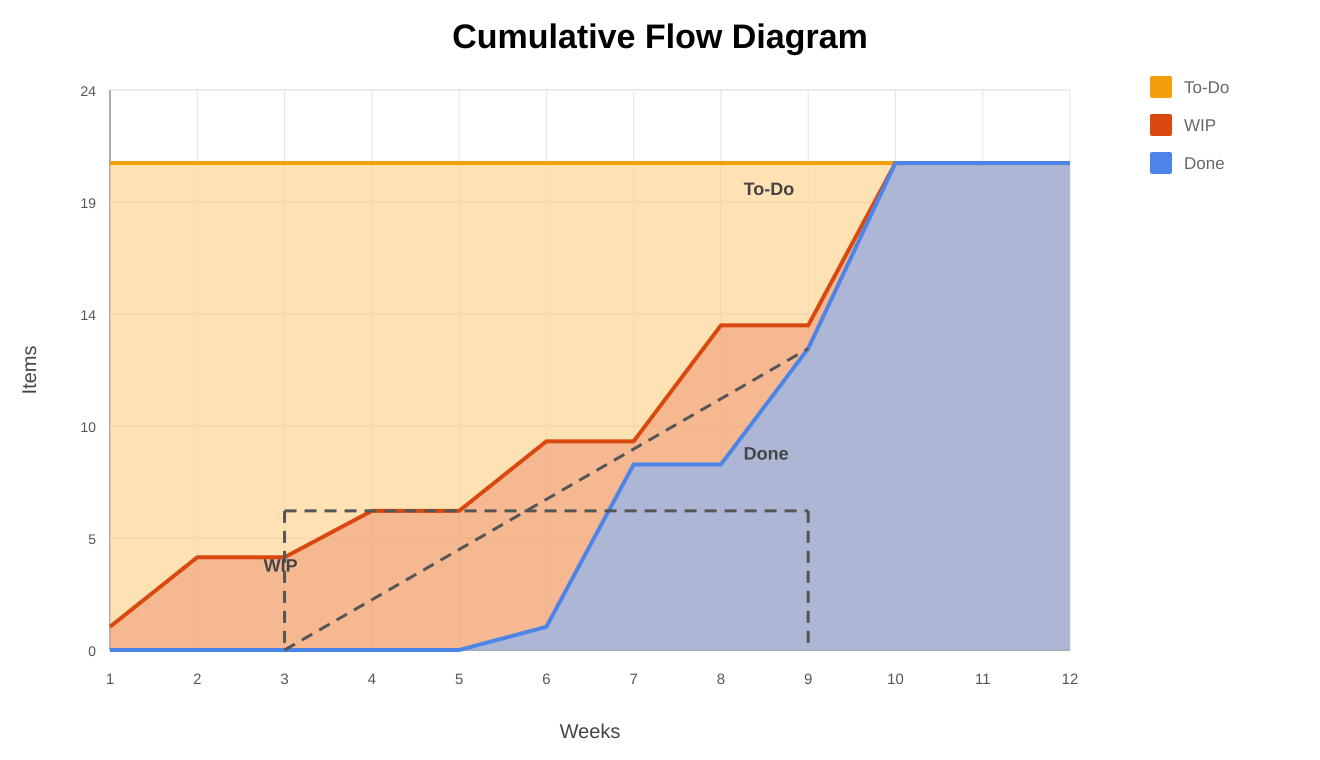
\includegraphics[width=0.92\linewidth]{figures/cfd.png}
\end{center}

The connected story here is that work did not close uniformly. The CFD shows that a significant amount of scope remained in progress until later sprints, which means the team was relying on staged maturity: foundation first, workflow next, operational modules after that, and only then full integration. That makes sense for this project, but it also explains why Sprint 5 felt dense.

\subsection{Throughput Report}
Throughput was measured at two levels: completed work items by sprint and feature-delivery behavior by git history. The project-wide sprint throughput shape is shown below.

\begin{center}
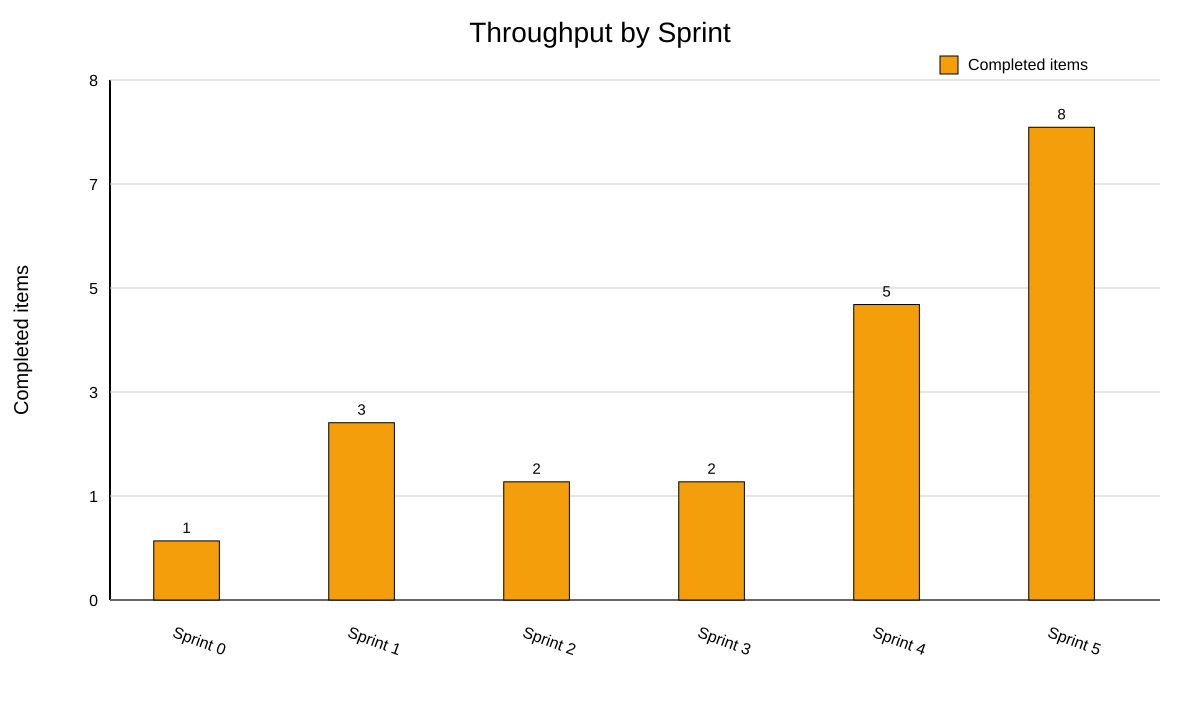
\includegraphics[width=0.92\linewidth]{figures/throughput.png}
\end{center}

The important observation is that throughput increases toward Sprint 4 and Sprint 5 instead of being flat across the semester. That is a real signal, not noise. It tells us that once the backend architecture stabilized, the team accelerated feature closure. The cost of that acceleration, however, was a more compressed integration phase.

\subsection{Project Burndown and Burnup}
Because the prompt explicitly allows telling the test and project story in our own way, we chose project-wide burn charts instead of a narrow single-sprint chart. This gives a more honest picture of how scope accumulated and how completion caught up over time.

\begin{center}
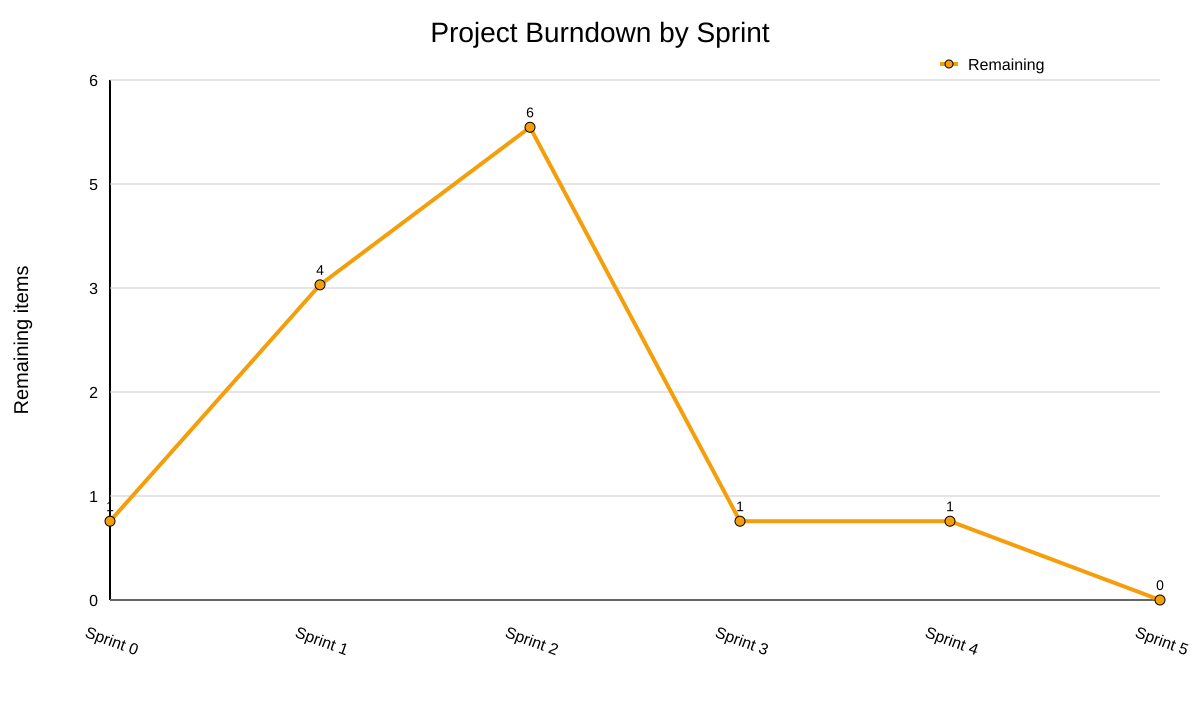
\includegraphics[width=0.92\linewidth]{figures/burndown.png}
\end{center}

\begin{center}
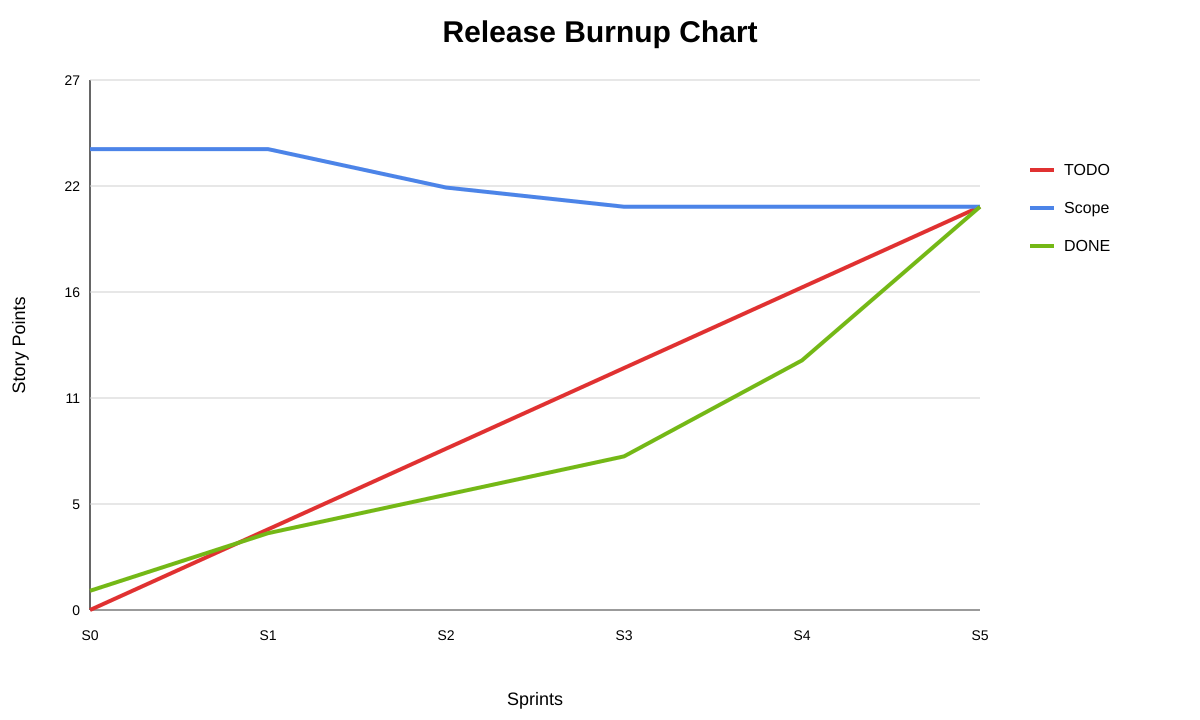
\includegraphics[width=0.92\linewidth]{figures/burnup.png}
\end{center}

The burndown and burnup together tell a coherent story. Scope expanded in a planned way from Sprint 0 through Sprint 5, but completion rose in steps rather than smoothly. That means the main process weakness was not uncontrolled scope growth; it was late visible closure. This distinction matters because the mitigation is not to reduce ambition, but to make integration and documentation visible earlier.

\subsection{Additional Metric 1: Code Churn}
Code churn was measured from git additions and deletions aggregated by week.

\begin{center}
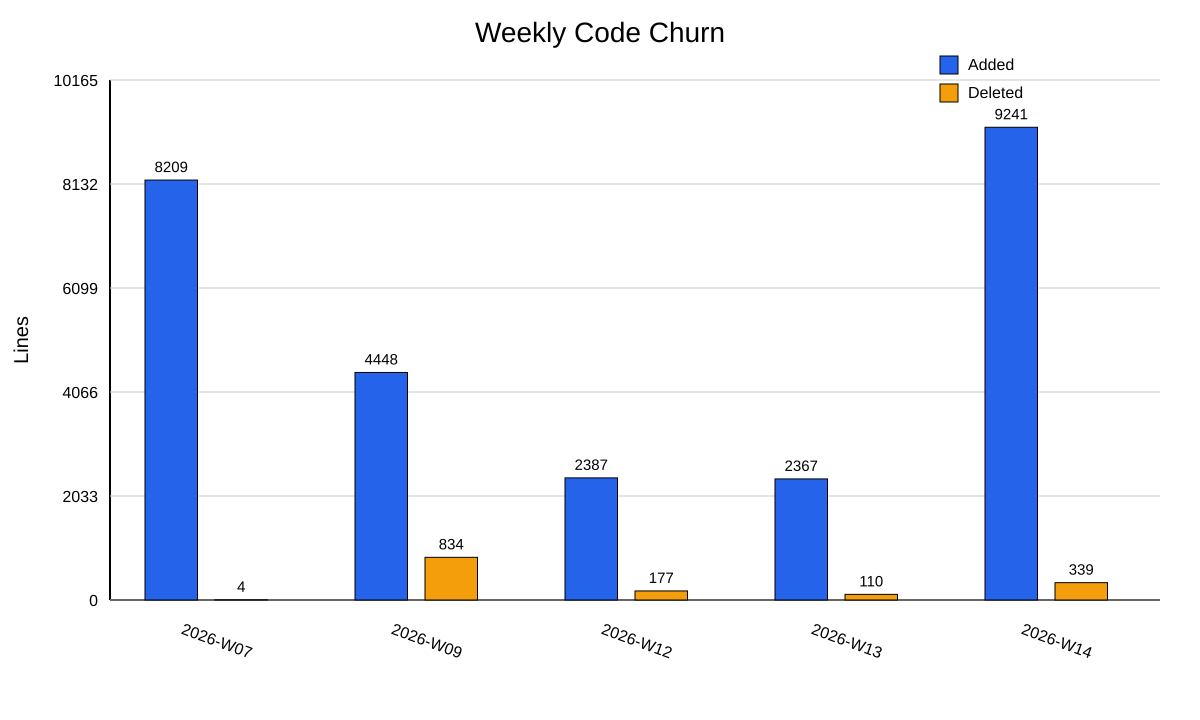
\includegraphics[width=0.92\linewidth]{figures/code_churn.png}
\end{center}

The project had its highest churn during the phase where the backend moved from setup to real implementation. Later churn remained substantial during operational-module work and Sprint 5 integration. This is healthy as long as it is paired with tests and documentation. Without that pairing, churn would instead be a sign of instability.

\subsection{Additional Metric 2: Test and Performance Story}
The second additional metric is a combined quality story: pass rate and NFR timing compliance. The repository currently documents 48 categorized test cases in the CSV, all marked PASS, while the broader smoke automation has grown to 59 checks.

\begin{center}
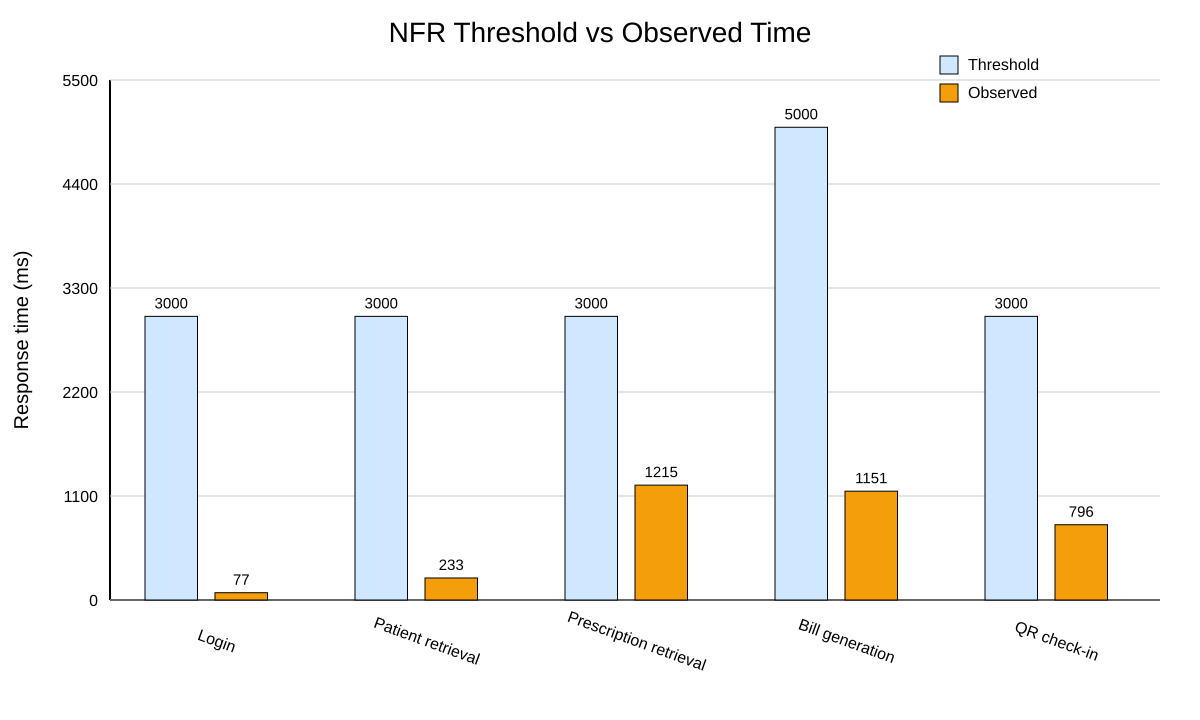
\includegraphics[width=0.92\linewidth]{figures/nfr.png}
\end{center}

The chart shows that all observed timings remain comfortably inside the stated thresholds. Login, patient retrieval, prescription retrieval, bill generation, and QR check-in all stay within the bounds defined in the project’s testing narrative. The positive result is that functional maturity and performance sanity were achieved together. The caution is that documentation synchronization became a project risk once the smoke suite grew beyond the 48-case CSV.

\section{Section II: Risk Analysis}
\subsection{Why a 5x5 Matrix Fits This Project}
The attached template suggests a classic 5x5 probability-impact matrix. That is appropriate here because the PHC system is not dominated by one catastrophic technical unknown; instead, it faces multiple moderate-to-high operational and integration risks that need prioritization. We therefore use the following scale. \textbf{Probability:} 1 = Rare, 2 = Unlikely, 3 = Moderate, 4 = Likely, 5 = Almost Certain. \textbf{Impact:} 1 = Insignificant, 2 = Minor, 3 = Significant, 4 = Major, 5 = Severe. \textbf{Risk score:} \(Probability \times Impact\).

\subsection{5x5 Risk Matrix}
\begin{center}
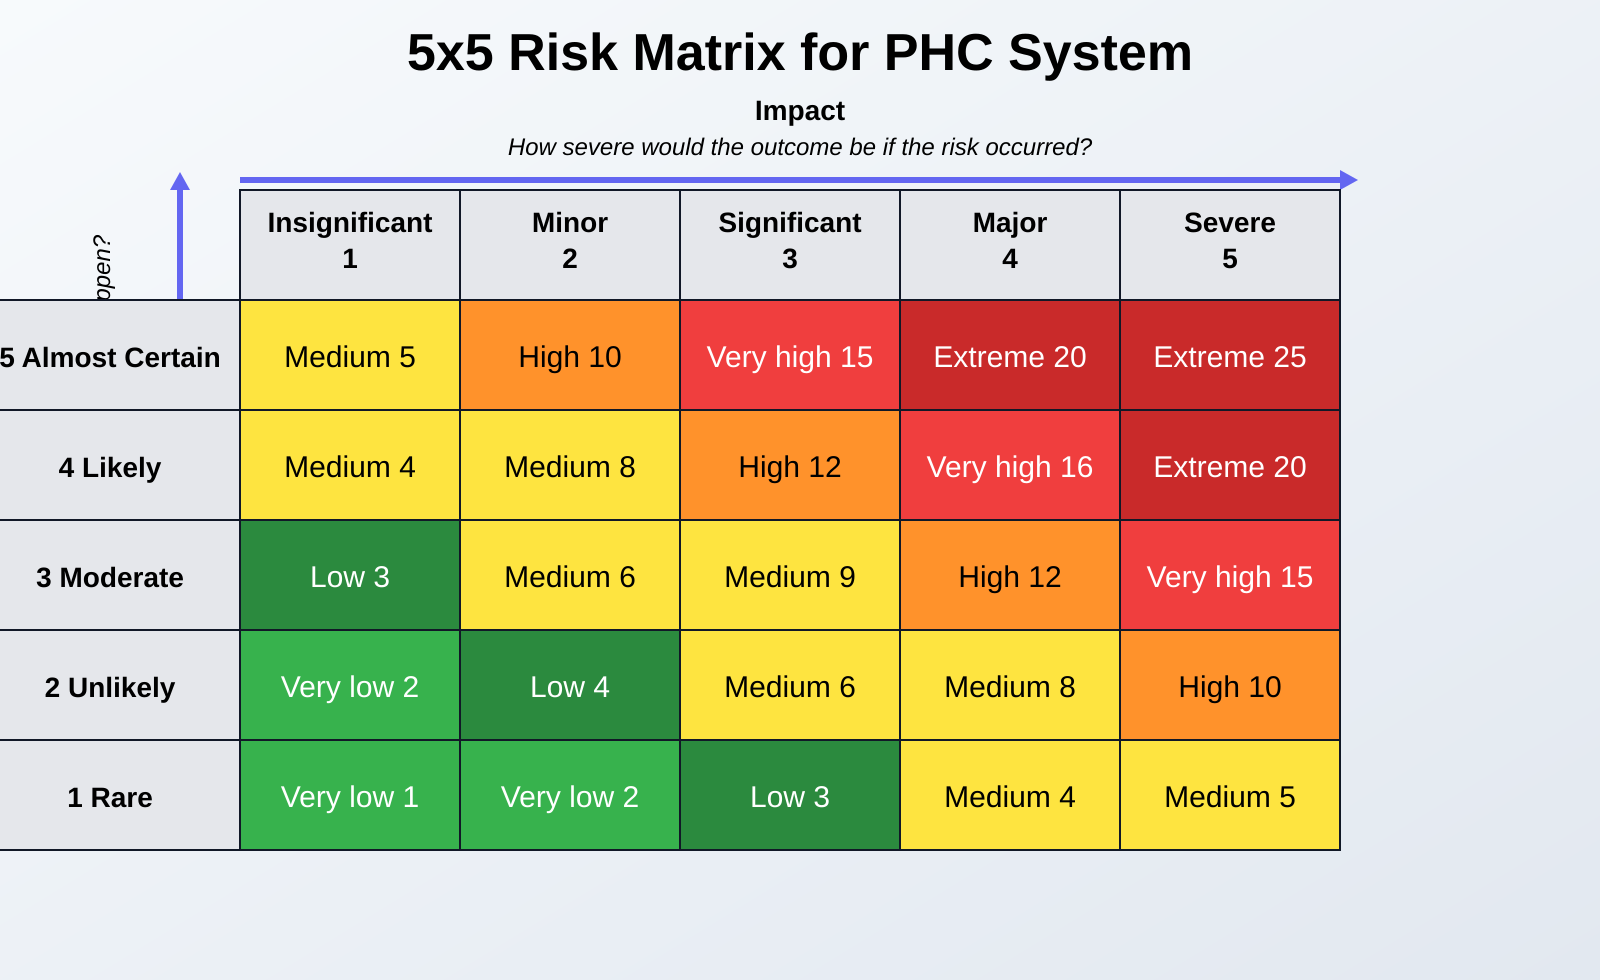
\includegraphics[width=0.98\linewidth]{figures/risk_matrix.png}
\end{center}

\subsection{Project-Specific Risk Register}
The matrix above is only the template. The real value comes from placing our own project risks into it.

\begin{center}
\rowcolors{2}{SoftGray}{white}
\begin{longtable}{|p{0.8cm}|p{4.1cm}|p{0.8cm}|p{0.8cm}|p{1.2cm}|p{6cm}|}
\hline
\rowcolor{SoftBlue}
\textbf{ID} & \textbf{Risk} & \textbf{P} & \textbf{I} & \textbf{Score} & \textbf{Mitigation logic} \\
\hline
R1 & Cross-module integration regression across visits, lab, pharmacy, billing, and notifications & 4 & 4 & 16 & Keep transaction boundaries, maintain the E2E runner, and use smoke tests before documentation freeze. \\
\hline
R2 & Late sprint convergence hides unfinished work until very close to milestone deadlines & 4 & 4 & 16 & Break work into smaller visible backlog items and insist on earlier integration checkpoints. \\
\hline
R3 & LDAP or authentication instability blocks role-based access and demos & 3 & 5 & 15 & Use Dockerized local LDAP, explicit 401/503 behavior, seeded test users, and auth verification in smoke and E2E tests. \\
\hline
R4 & Database migration or shared-model change damages visit-linked consistency & 3 & 5 & 15 & Use Prisma migrations only, preserve idempotent seed flow, and validate \texttt{migrate deploy}. \\
\hline
R5 & Documentation drift between README, TESTING, smoke counts, CSV evidence, and report content & 4 & 3 & 12 & Treat docs as first-class deliverables and regenerate report data from scripts rather than manual counting. \\
\hline
R6 & Frontend lag leaves the project backend-complete but demo-incomplete & 4 & 3 & 12 & Freeze backend scope unless blocked and turn the stable API into role dashboards in Sprint 6. \\
\hline
R7 & RBAC error exposes medical data to the wrong role & 2 & 5 & 10 & Preserve route guards, add more RBAC tests, and keep patient-only endpoints clearly separated. \\
\hline
R8 & Performance and security hardening remain behind functional completion & 2 & 4 & 8 & Reserve Sprint 7 for hardening, load checks, and deployment preparation rather than new features. \\
\hline
\end{longtable}
\end{center}

The probability assumptions here are not arbitrary. They are tied to what the repository already showed. For example, documentation drift is marked likely because the project already developed a mismatch between the 48-case CSV and the larger smoke suite. Late sprint convergence is marked likely because the burndown/burnup story shows completion clustering near Sprint 5 closeout.

\section{Section III: Mapping Risk Mitigation to Sprint Planning}
This final section is where the report becomes a connected story instead of a list of charts. The project did not merely \emph{have} risks; it already responded to them through sprint ordering.

\begin{center}
\rowcolors{2}{SoftGray}{white}
\begin{tabular}{|p{1.3cm}|p{4cm}|p{7.7cm}|}
\hline
\rowcolor{SoftBlue}
\textbf{Sprint} & \textbf{Main risks addressed} & \textbf{How mitigation entered the backlog} \\
\hline
Sprint 0 & Scope ambiguity & Initial SRS revisions and UML work narrowed the project away from ambulance-style scope and toward a PHC-centered system. \\
\hline
Sprint 1 & Auth, storage, and requirement instability & Authentication, schema, and patient profile work were pulled first so all later modules had a stable identity and persistence base. \\
\hline
Sprint 2 & Workflow inconsistency & The team implemented visit lifecycle and doctor availability before prescriptions or labs, reducing downstream rework risk. \\
\hline
Sprint 3 & Clinical-module fragmentation & Prescriptions and lab requests were added only after consultation and queueing existed, which kept clinical flows coherent. \\
\hline
Sprint 4 & Transaction and operational risk & Billing and check-in were implemented with transaction-safe design, and operational modules were integrated without changing the visit-centric backbone. \\
\hline
Sprint 5 & Integration, documentation, auth hardening & Admin modules, notifications, E2E flow validation, API documentation, and real local LDAP support were explicitly added as mitigation work, not just as features. \\
\hline
Sprint 6 & Backend/UI imbalance & The current plan is to convert the stable API into role dashboards rather than reopen backend scope. \\
\hline
Sprint 7 & Release-readiness risk & Testing depth, RBAC verification, security hardening, load checks, and deployment preparation are reserved for the stabilization sprint. \\
\hline
\end{tabular}
\end{center}

This is the clearest way to tell the project story: the sprint order itself is a risk-mitigation strategy. The team did not just build modules in arbitrary order. It used ordering to reduce structural risk first, workflow risk next, operational risk later, and integration risk near backend closeout.

\section{Conclusion}
The PHC Integrated Digital System now has a strong backend story backed by measurable evidence. The COCOMO estimate places it in a meaningful engineering range, the Halstead and function-point results show non-trivial complexity, the flow and throughput charts show how work matured over time, and the test/performance data shows that the backend is not only large enough to matter but also stable enough to demonstrate.

The deeper conclusion, however, is about project control. The team’s real challenge is no longer \emph{whether} it can build the backend. It already has. The real challenge is how to convert that backend maturity into a coherent final product by keeping documentation aligned, making Sprint 6 visible, and using Sprint 7 for hardening instead of feature creep. That is why this report tells one connected story: metrics, risks, and sprint planning are not separate topics in this project. They are three views of the same development reality.

\section*{Progress Tracker}
\href{https://docs.google.com/spreadsheets/d/1xLa2L8eWv8gfrIwPXrnImF8uManlRlRwRp3ksSOVI9E/edit?usp=sharing}{Project tracker spreadsheet}

\section*{AI Use Disclosure}
AI assistance was used for report drafting, chart generation scripts, and workbook/report consolidation. All computed values, repository references, risk judgments, and final narrative were manually reviewed against the current project artifacts.

\end{document}
